\section{Methodology} The methodology is structured into three sequential phases, each addressing a distinct part of our multi-dimensional analysis. In Phase I we develop a holistic taxonomy-based representation of security faults. In Phase II we construct an automated data-extraction pipeline to collect and aggregate vulnerability records. In Phase III we perform exploratory analysis on the dataset and derive a hierarchical classification scheme based on observed patterns. Each phase builds on the previous, ensuring a coherent flow from abstract taxonomy to concrete classification.

\subsection{Holistic Representation of Security Faults} \textbf{Aim:} Synthesize existing vulnerability taxonomies into a unified attribute schema. This phase consolidates diverse security-fault taxonomies (e.g. language-specific faults, technology categories, architectural layers, and root-cause taxonomies) to create a comprehensive representation of vulnerability attributes.
\newline

%Landwehr’s multi-dimensional foundation: NASA retains genesis (coding errors) and time (phase analysis) but replaces location with subsystem concentration (90% in 2–4 subsystems).

%Piessens’ causal focus: Extends this by linking vulnerability causes to lifecycle phases (e.g., Exception Management flaws stemming from ambiguous error handling during implementation).

%Weber’s tool-oriented schema: Complements by providing empirical data to train static analyzers on NASA’s dominant CWEs (e.g., Risky Values).


\textbf{Steps:}

\begin{itemize}
    \item \textbf{Survey taxonomies.} We collect relevant taxonomies from literature and standards. For example, language- and platform-based taxonomies (e.g. C/C++ errors vs. Web app issues), technology-focused taxonomies (e.g. web, database, OS level), software-layer taxonomies (e.g. presentation vs. business logic), and root-cause taxonomies (e.g. input validation, memory corruption).
    \item \textbf{Identify attributes.} From each taxonomy we extract key attributes (e.g., "Buffer Overflow", "SQL Injection", "Cross-Site Scripting", "Race Condition", etc.) and note which taxonomies include each attribute.
    \item \textbf{Create Unified Attribute Matrix.} We compile these attributes into a matrix with rows as example attributes and columns indicating taxonomy source. Table~\ref{tab:attribute-matrix} (excerpt below) illustrates how attributes map across taxonomies. This "Unified Attribute Matrix" highlights overlaps and gaps, guiding later analysis.
\end{itemize}

\begin{table}[ht!]
    \centering
    \caption{Unified Attribute Matrix}
    \label{tab:attribute-matrix}
    \begin{tabular}{lcccc}
        \hline
        \textbf{Attribute} & \textbf{Lang-based \cite{cwe_list}} & \textbf{Tech-based \cite{Khwaja2020ASF}} & \textbf{Layer \cite{sa_nikolai}} & \textbf{Root Cause \cite{Shahriar2012MitigatingPS}} \\
        \hline
        Buffer Overflow & \checkmark & \checkmark & & \checkmark \\
        SQL Injection & & \checkmark & \checkmark & \\
        Cross-site Scripting & & \checkmark & \checkmark & \\
        Privilege Escalation & \checkmark & & & \checkmark \\
        Invalid Input & & & & \checkmark \\
        \hline
    \end{tabular}
\end{table}

This phase yields a consolidated schema of security fault attributes that will guide data collection and later classification. In particular, the unified list of attributes becomes the basis for labeling and grouping vulnerabilities in subsequent phases.

\subsection{Collecting and Analyzing Data for Vulnerability Profiling} 

Figure~\ref{fig:extraction-pipeline} gives an overview of our multi-stage data processing pipeline for constructing a large-scale, multi-dimensional vulnerability dataset. This pipeline guides the systematic collection, enrichment, and consolidation of vulnerability data to support empirical profiling of security faults across software ecosystems. Our methodology integrates heterogeneous sources and leverages custom-developed tools to ensure consistency, traceability, and analytical utility of the resulting dataset.

The pipeline begins with \textbf{selecting application-level \ac{CVE}s} enriched with code-relevant weaknesses. Drawing from over two decades of records in the \ac{NVD}, we apply a reproducible filtering process that isolates vulnerabilities affecting application-layer software. This filtering is implemented using a suite of internally developed Python packages that enforce strict quality and relevance constraints, enabling a focused dataset suitable for downstream analysis. That includes \texttt{nvdutils}\footnote{\texttt{nvdutils}: A Python package for parsing, representing, filtering, and analyzing NVD data.}, \texttt{cpelib}\footnote{\texttt{cpelib}: A Python package for parsing, representing, and filtering the NVD \ac{CPE} Dictionary.}, and \texttt{pydantic-cwe}\footnote{\texttt{pydantic-cwe}: A Python package for modeling \ac{CWE} entries as Pydantic objects.}. 

Next, we perform \textbf{software type inference} to categorize affected products according to their functional roles—such as libraries, servers, or web applications. This classification enables more granular comparisons of vulnerability patterns across different categories of software. By analyzing metadata from the CPE dictionary and reconciling with curated external datasets, we construct a typology of software artifacts that improves the contextual interpretability of observed vulnerabilities.

To enhance this profiling further, we develop a methodology for \textbf{mapping software products to programming languages}. This stage involves inferring implementation languages through a combination of structured data extraction, curated mappings, and heuristics. Associating each product with a language (or set of languages) allows us to investigate correlations between implementation choices and vulnerability types, addressing critical questions about the security implications of language ecosystems.

In the final stage, we perform \textbf{dataset consolidation}, merging enriched vulnerability records into a unified dataset. Each CVE is linked to a representative software product and annotated with associated metadata, including inferred language(s), software type, and CWE classification. This dataset—covering over 60,000 CVEs—enables visualization and analysis of security trends, such as frequent CWE-language pairings or high-risk software categories. A final co-occurrence analysis, visualized via a Sankey diagram, reveals dominant structural patterns in vulnerability distributions, laying the foundation for data-driven insights into the socio-technical determinants of software security.

\subsubsection{CVE and CWE Selection Criteria}
We restricted the analysis exclusively to application-level vulnerabilities. This was operationalized using the configuration layer to include only products categorized under the "Application" part of the \ac{CPE} taxonomy. This decision aligns with the research focus on software-level flaws rather than infrastructure or hardware vulnerabilities. To exclude incomplete, misleading, or invalid entries, the \ac{CVE} filtering layer was configured to accept only entries marked as valid. Vulnerabilities flagged as Rejected, Deferred, Disputed, or Unsupported were automatically excluded. This ensures that the selected CVEs reflect accepted and actionable disclosures.

The dataset was further refined by retaining only CVEs associated with a single, deterministically selected weakness, thereby enhancing analytical precision and minimizing classification ambiguity. For CVEs mapped to multiple CWEs, a structured resolution strategy was applied based on guidance from MITRE’s CWE usage recommendations. Each weakness was assigned a score according to its abstraction level, with more specific weaknesses prioritized, ordered from most to least specific as Variant > Base > Class > Compound > Chain. Additionally, weaknesses designated as “Primary” in the NVD schema were assigned an extra weight to further promote their selection. The CWE with the highest combined score was retained per CVE, ensuring consistency and mitigating noise from auxiliary or less informative mappings. To preserve semantic integrity and analytical relevance, weaknesses marked as deprecated or annotated with mapping notes falling outside the “Allowed” or “Allowed-with-Review” categories were excluded from consideration. This methodology reflects best practices in root-cause mapping and aligns with the CWE program’s emphasis on using precise, non-discouraged mappings to represent the dominant weakness per vulnerability instance.

\subsubsection{Identification of Code-Relevant Weaknesses}
To maintain thematic consistency with software implementation-level issues, we preselected a curated subset of \ac{CWE}s that exhibit strong evidence of code-relevance. This subset was identified by examining the nature of each weakness's lifecycle placement, detection modalities, presence of example code, and alignment with known software attack patterns:

\begin{itemize}
    \item \textbf{Lifecycle Placement}: CWEs with introduction or mitigation phases classified as "Implementation" were prioritized, acknowledging that the origin or resolution of such weaknesses typically occurs within the software development lifecycle.
    \item \textbf{Detection Modalities}: CWEs amenable to automated or semi-automated static or dynamic analysis were included, consistent with scalable security tooling strategies.
    \item \textbf{Code Examples}: Weaknesses accompanied by reference implementations or exploit examples were retained as they provide tangible manifestations of the underlying flaw.
    \item \textbf{Attack Pattern Alignmen}t: CWEs linked to software attack pattern IDs from the CAPEC database were included to reinforce the practical exploitability of the weakness.
\end{itemize}

\begin{figure}[!h]
	\centering
    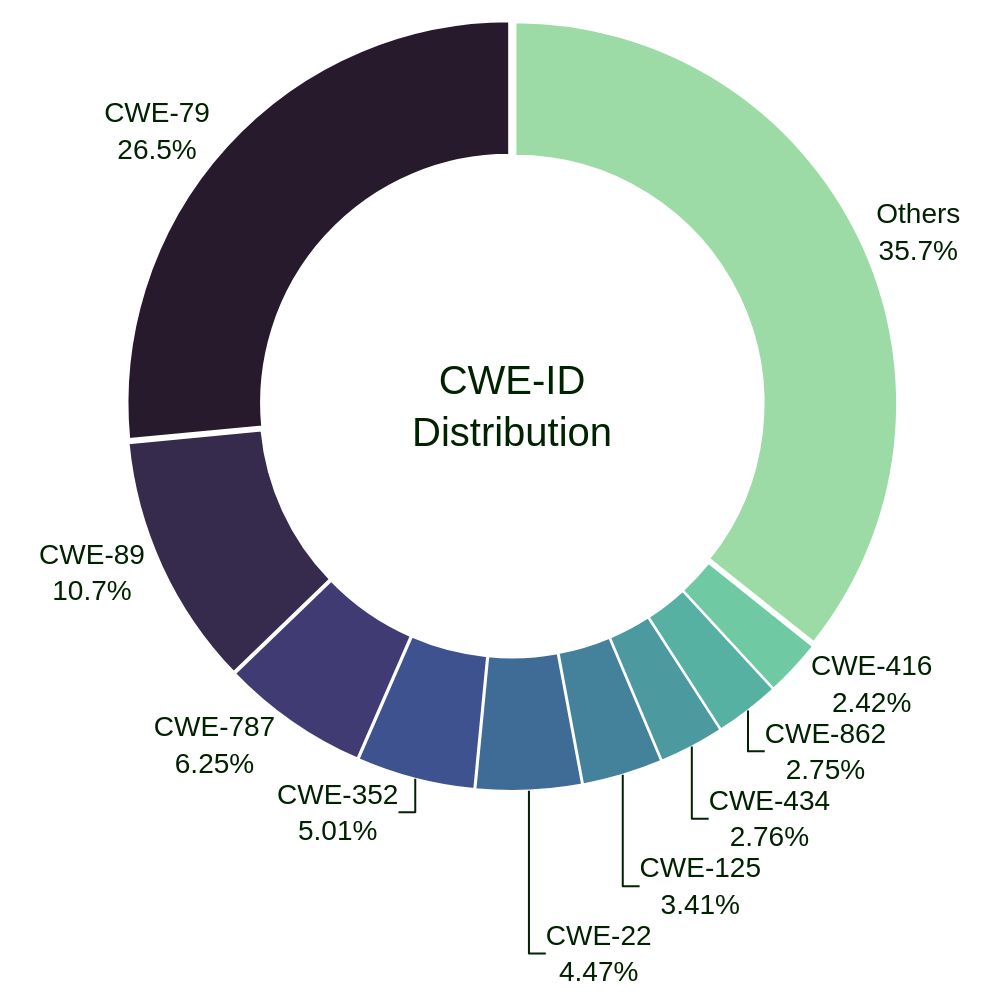
\includegraphics[width=0.55\textwidth]{figures/chapter_2/cwe_distribution_donut.png}
	\caption{Distribution of CWE-IDs in the Selected CVE Set}
	\label{fig:cwe_distribution}
\end{figure}

The final script, executed over the full JSON feed of the NVD dataset, yielded 78,620 CVEs conforming to the above criteria. Each entry was recorded alongside its dominant CWE identifier. The top 25 CWEs accounted for over 83\% of the total dataset, underscoring the concentration of application vulnerabilities around a core set of recurring weakness types. As shown in Figure~\ref{fig:cwe_distribution}, this concentration is particularly evident in the dominance of web application vulnerabilities, with CWE-79 (Cross-site Scripting) representing 26.5\% of all entries, followed by CWE-89 (SQL Injection) at 10.7\%. Memory safety issues also feature prominently, with CWE-787 (Out-of-bounds Write) accounting for 6.25\% of vulnerabilities. Other significant categories include CWE-352 (Cross-Site Request Forgery) at 5.01\% and CWE-22 (Path Traversal) at 4.47\%, while the remaining CWE types collectively comprise 35.7\% of the dataset. This distribution enhances the tractability of downstream analyses and enables longitudinal and categorical insights into software vulnerability trends.

\subsubsection{Software Type Inference Based on CPE Metadata}
The first stage involves labeling software entries in the CPE dictionary based on three complementary heuristics: (1) the target platform the software is associated with, (2) keywords in the product name, and (3) domain names in associated URLs.

\begin{itemize}
    \item \textbf{Target Platform Mapping}: Certain CPE entries specify a \texttt{target\_sw} field, which indicates the environment or platform that the software targets. We maintain a mapping from known platforms (e.g., wordpress, drupal, jira) to high-level software types such as extension, library, or framework. This mapping assumes that targeting a specific ecosystem typically implies a consistent functional role (e.g., WordPress-targeting software is likely a plugin or extension).
    \item \textbf{Product Name Keywords}: For entries lacking an informative target platform, we analyze the product name using a curated list of keywords associated with software types. Terms like plugin, sdk, module, and api are indicative of roles such as extension or library. This lexical heuristic captures semantic cues commonly embedded in naming conventions.
    \item \textbf{Reference Domain Analysis}: When a product includes external references (URLs), we extract domain names and match them against a precompiled mapping of known software directories and marketplaces (e.g., marketplace.visualstudio.com, patchstack.com). These sources are generally tied to specific types of software (e.g., extensions), and thus offer additional contextual signals.
\end{itemize}

Each of these signals contributes a possible label. If more than one label is inferred for a product, a resolution process is applied to select the most appropriate one.


\subsubsection{Label Reconciliation and Conflict Resolution}
To strengthen the reliability of our labels, we align them with a manually labeled dataset from prior research by Ezenwoye \textit{et al.}~\cite{Ezenwoye2020ClassifyingCS}. This dataset includes vendor and product pairs annotated with software types. After cleaning and normalizing the dataset (e.g., removing the category \texttt{operating system} and standardizing labels such as converting web application to \texttt{web\_app}), we merge it with our inferred CPE dataset using vendor and product identifiers.

Merged entries may contain divergent labels from the CPE-based inference and the research dataset. In such cases, we apply a deterministic rule-based function to select one label based on the observed combination. These rules are designed to maintain consistency and prefer more specific labels when appropriate. For instance, if the research dataset labels a product as a framework, but our inference suggests library or extension, we retain the more granular label. In cases where the CPE-inferred label is based solely on a reference URL (indicated by a \texttt{\_ref} suffix), we prioritize that label if no better alternative exists.

\begin{figure}[!h]
	\centering
    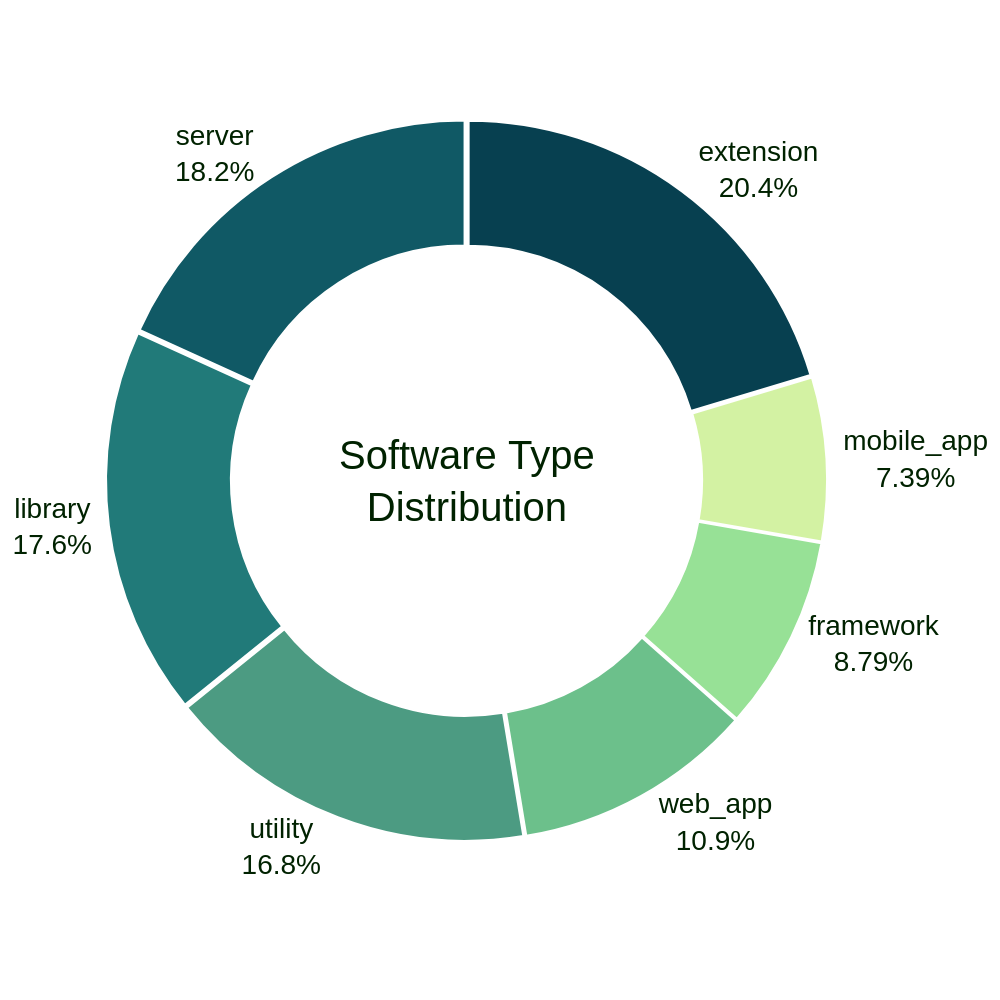
\includegraphics[width=0.55\textwidth]{figures/chapter_2/software_type_distribution_donut.png}
	\caption{Distribution of Software Type in the Labelled Set of Products}
	\label{fig:software_type_distribution}
\end{figure}

Applying this classification methodology, we successfully labeled 34,575 unique software products with a corresponding software type. Figure~\ref{fig:software_type_distribution} depicts the resulting distribution of functional roles: extension (20.35\%), server (18.22\%), library (17.57\%), utility (16.82\%), web\_app (10.86\%), framework (8.79\%), and mobile\_app (7.39\%). This distribution highlights the prevalence of modular and infrastructure-supporting components such as extensions and libraries, as well as the substantial representation of utility and server software. These labeled categories form the foundation for our subsequent analyses of vulnerability types, enabling us to associate specific fault patterns with software of varying functional scopes and operational contexts.


\subsubsection{Mapping Software Products to Programming Languages}
We begin by leveraging the publicly available SQLite database from the  \texttt{purl2cpe} SCANOSS project~\footnote{\texttt{purl2cpe} - \url{(https://github.com/scanoss/purl2cpe)}}, which maps package URLs (PURLs) to the standardized \ac{CPE} identifiers. This dataset serves as a bridge between open-source software packages and the structured taxonomy used in vulnerability repositories. For each CPE entry, we extract associated PURLs and use predefined heuristics to infer programming languages. Specifically, we apply a static mapping from PURL types to canonical languages (e.g., pypi → Python, maven → Java). This heuristic captures common package ecosystems and provides a baseline for language classification.

However, not all packages yield direct mappings, particularly when repositories span multiple technologies or lack explicit package type indicators. To extend coverage, we incorporate language metadata from GitHub repositories linked to the PURLs. This step employs a custom Python package developed for the study, coined \texttt{gitlib}~\footnote{\texttt{gitlib} - \url{https://github.com/epicosy/gitlib}}, which interfaces with the GitHub API to identify the dominant programming language of a repository. The process includes parsing repository links, aggregating language-specific byte counts, and applying prioritization heuristics on a classification scheme during language inference when a dominant language is ambiguous. A final language label is assigned for each product, incorporating both direct mappings and inferred metadata.

\subsubsection{Programming Language Classification for Software Product Mapping}
To accurately associate software products with their underlying programming languages, we classify programming languages into two main categories: \textbf{primary} and \textbf{secondary} languages. This distinction plays a crucial role in determining the most representative language for a given software product.

\textbf{Primary languages} encompass general-purpose programming languages capable of supporting the development of full-featured software systems. These languages are Turing-complete and are widely used across various domains, including web development, systems programming, and application development. When identifying a product's language, this category is prioritized due to its broad applicability and higher likelihood of representing the product's core logic. Examples of primary languages include: 

\begin{itemize}
    \item \textbf{Popular web and backend languages}: PHP, Python, Java, JavaScript;
    \item \textbf{Systems and application programming}: C, C++, Rust, Go, C\#;
    \item \textbf{Scripting and object-oriented languages}: Ruby, Kotlin, Swift, TypeScript;
    \item \textbf{Functional and academic languages}: Haskell, Scala, Clojure, Erlang;
    \item \textbf{Legacy and enterprise languages}: Visual Basic, COBOL, Fortran, Ada;
\end{itemize}

\textbf{Secondary languages} are also executable but are tailored to specific domains or computational tasks. While they may appear frequently in repositories, their presence is often supplementary to the main application logic. As such, they are considered only when no suitable primary language can be confirmed. Examples of secondary languages include:

\begin{itemize}
    \item \textbf{Database and query languages}: SQL, TSQL, PLpgSQL;
    \item \textbf{Statistical and scientific computing}: R, MATLAB, Mathematica;
    \item \textbf{System scripting and automation}: Shell, PowerShell;
    \item \textbf{Specialized domains}: Solidity (blockchain), TeX (typesetting);
\end{itemize}

\subsubsection{Product Language Prioritization Heuristics}
When analyzing GitHub repositories associated with software products, the classification introduced above is used to guide language selection, particularly in cases where a software repository contains code in multiple languages. The prioritization heuristics for language selection have the following order of preference:

\begin{enumerate}
    \item The main language, if it belongs to the primary category;
    \item The second most-used language, if in the primary category;
    \item The main language, if in the secondary category;
    \item The second most-used language, if in the secondary category;
\end{enumerate}

This hierarchy reflects the assumption that primary languages are more likely to encapsulate the software's central functionality, while secondary languages contribute auxiliary capabilities. 
%This prioritization mechanism, embedded in the GitHub repository analysis component, supports the broader objective of uncovering meaningful correlations between software characteristics and observed security faults. 

\begin{figure}[!h]
	\centering
    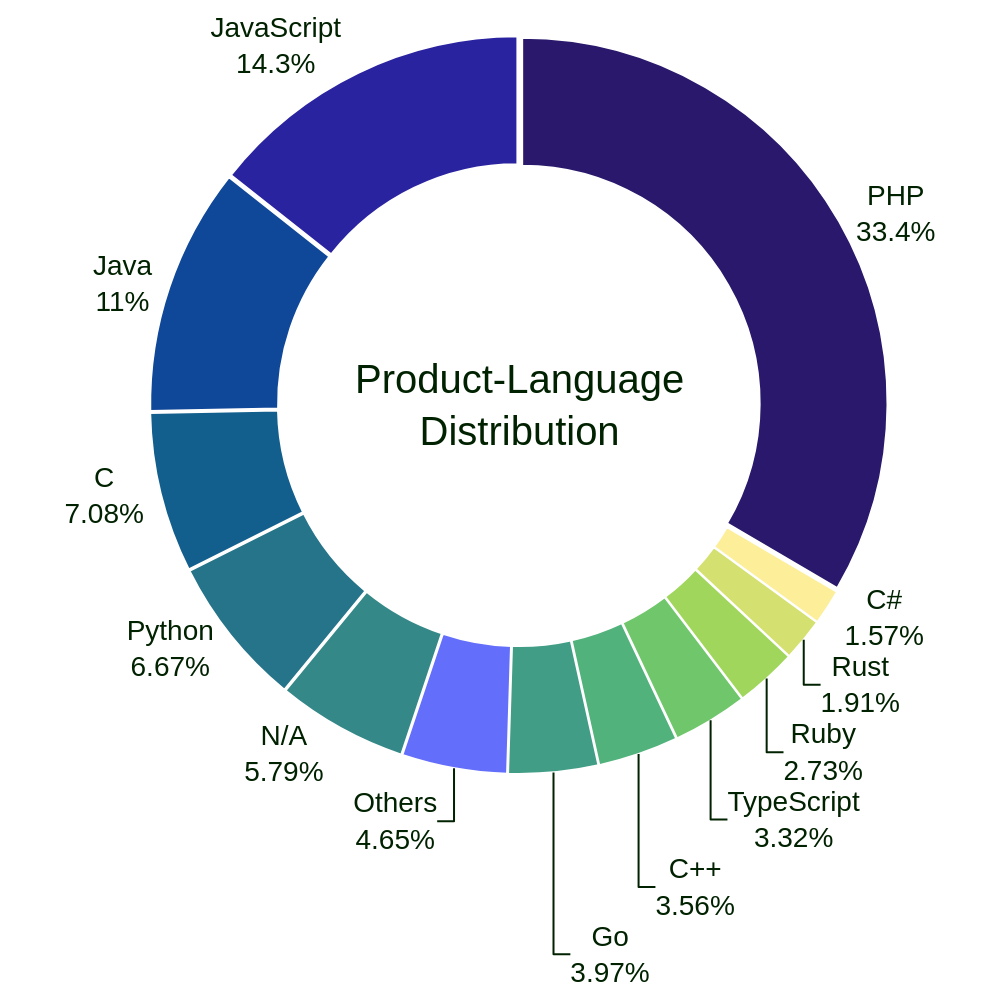
\includegraphics[width=0.55\textwidth]{figures/chapter_2/product_language_distribution_donut.png}
	\caption{Distribution of Programming Language in the Labelled Set of Products}
	\label{fig:product_language_distribution}
\end{figure}

The integration of package metadata with repository-level analysis produces a dataset of 14,927 unique entries that maps software products to their primary implementation languages, covering a diverse set of 63 programming languages. Figure~\ref{fig:product_language_distribution} illustrates that the resulting distribution of programming languages reflects prevailing trends in the open-source ecosystem. PHP emerges as the most common language, accounting for 33.4\% of the mapped products, followed by JavaScript (14.3\%), Java (11.0\%), and Python (6.7\%). Notably, 5.8\% of the entries could not be confidently assigned a language and are marked as "N/A." Other frequently observed languages include Go (4.0\%), C++ (3.6\%), TypeScript (3.3\%), Ruby (2.7\%), Rust (1.9\%), and C\# (1.6\%), with the remaining 4.6\% distributed among a long tail of less common languages. This language-labeled dataset forms the basis for subsequent analyses examining the intersection of programming language and vulnerability characteristics.

\subsubsection{Inferring Programming Languages from Vulnerability Descriptions}
To enrich the dataset with more reliable language annotations and to better support downstream analysis, we incorporate a heuristic-based text analysis technique aimed at identifying programming languages directly from CVE descriptions. This step complements the existing product-language mapping by addressing cases where the product metadata alone may be ambiguous or unavailable.

The implemented approach scans CVE descriptions for filenames with known file extensions, drawing on a curated list of language extension mapping based on the previous programming language classification. By extracting these filenames and counting the frequency of their associated extensions, we determine the most probable language used in the context of the reported vulnerability. A conservative matching strategy ensures that only likely file references (e.g., \texttt{index.php}, \texttt{main.py}) are considered, while false positives such as domain names and non-code artifacts are filtered out using regular expressions and URL parsing logic.

\subsubsection{Dataset Consolidation}
We infer the programming language directly from descriptions in 11,924 of the 78,620 CVEs, substantially enhancing both the coverage and specificity of language attribution. These inferred labels are then integrated with the previously constructed datasets, which include the CVE-ID, CWE-ID, and detailed product metadata such as vendor, software type, and package source. To associate each CVE with the most representative software product, we apply a scoring heuristic that prioritizes certain software categories, such as libraries over web applications, and gives preference to GitHub-hosted packages. The result is a unified dataset where each entry corresponds to a single vulnerability and is enriched with attributes including CVE ID, CWE ID, vendor, product, software type, and programming language. In total, the consolidated dataset comprises 61,654 CVEs, of which 41,007 are linked to products with known metadata.

\begin{figure}[!h]
	\centering
    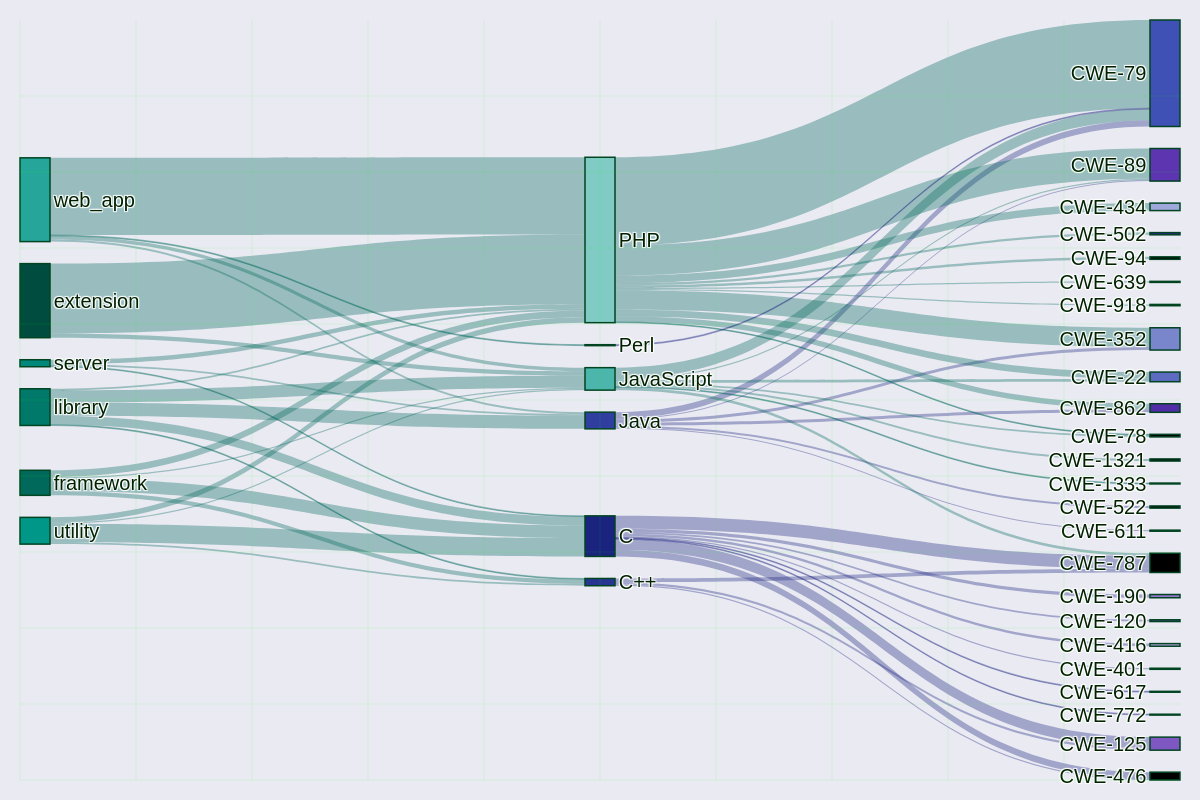
\includegraphics[width=1\textwidth]{figures/chapter_2/sankey_software_language_cwe.png}
	\caption{Sankey Diagram with the Relationships Among Attributes}
	\label{fig:sakney_attributes}
\end{figure}

To highlight common patterns, we visualize the co-occurrence relationships among software types, programming languages, and CWEs (Common Weakness Enumerations) using a Sankey diagram. This diagram captures the most frequent triplets observed in the dataset. For instance, the most prevalent link involves PHP-based extensions affected by CWE-79 (Cross-site Scripting), with 2,375 such instances. Web applications written in PHP are similarly dominant, particularly in connection with CWE-79 (2,206 instances) and CWE-89 (SQL Injection, 1,046 instances). Other prominent trends include C utilities vulnerable to buffer overflows (CWE-787, 283 instances), and Java libraries linked to CWE-79 (224 instances) and CWE-352 (Cross-Site Request Forgery). These patterns underscore the relevance of language and software-type context in shaping vulnerability profiles. This dataset is an initial effort and offers a foundation for empirical vulnerability analysis, enabling nuanced exploration of how implementation choices relate to security outcomes.


%Table~\ref{tab:vuln-dataset} shows sample rows from the final dataset. These integrations leverage multiple tools and APIs to maximize coverage of relevant fields. 

%\begin{table}[h!]
%\centering
%\caption{Example rows from vuln\_master\_dataset.csv after data collection. Each entry includes CVE ID, project context, CWE class, and a brief description.}
%\label{tab:vuln-dataset}
%\begin{tabular}{llllp{4cm}}
%\hline
%\textbf{CVE} & \textbf{Project} & \textbf{CWE} & \textbf{Severity} & \textbf{Short Description} \\
%\hline
%CVE-2021-12345 & ProjectA & CWE-79 (XSS) & High & Stored XSS in user comments widget \\
%CVE-2020-67890 & ProjectB & CWE-89 (SQLi) & Medium & SQL injection in search query builder \\
%CVE-2019-11111 & ProjectC & CWE-119 (Overflow) & Critical & Buffer overflow in image parser \\
%... & ... & ... & ... & ... \\
%\hline
%\end{tabular}
%\end{table}

\subsection{Mapping Analysis Results to Classification Scheme} \textbf{Aim:} Analyze the collected data to identify recurring patterns and design a multi-level classification scheme for security faults. The goal is to move from raw data to insight, culminating in a hierarchical taxonomy (Dimension $\rightarrow$ Subclass $\rightarrow$ Example CWE) that reflects the observed diversity of vulnerabilities.
\newline

\textbf{Steps:}
\begin{itemize}
    \item \textbf{Exploratory Analysis.} We perform statistical and visual analyses on the dataset. This includes generating histograms of vulnerabilities by language, technology, and layer; heatmaps showing co-occurrence of attributes; and scatter plots for correlations (e.g. severity vs. time). These visuals help highlight the most prominent fault attributes and gaps.
    \item \textbf{Pattern extraction.} From the visualizations we identify recurring themes. For instance, we may observe that web-related vulnerabilities (CWE-79, CWE-89) cluster in the "Technology: Web" category, or that certain root causes (e.g. improper input validation, CWE-20) appear across multiple languages and frameworks.
    \item \textbf{Classification hierarchy design.} Guided by the unified attributes (from Phase I) and patterns, we construct a three-level classification. The top level ("Dimension") corresponds to our major analysis axes (e.g. {\em Programming Language}, {\em Technology Domain}, {\em Architectural Layer}, {\em Root Cause}). The second level ("Subclass") refines each dimension (e.g. for Language: {\em Web Languages} vs. {\em System Languages}). The third level lists concrete examples, typically specific CWE identifiers or vulnerability types (e.g. {\em CWE-79: XSS} under "Technology: Web"). An excerpt of this hierarchy is shown in Table~\ref{tab:classification}, and its conceptual organization is visualized in Figure~\ref{fig:classification-hierarchy}.
\end{itemize}

\begin{table}[h!]
\centering
\caption{Excerpt of the classification hierarchy (Phase III): Dimension $\rightarrow$ Subclass $\rightarrow$ Example CWE.}
\label{tab:classification}
\begin{tabular}{lll}
\hline
\textbf{Dimension} & \textbf{Subclass} & \textbf{Example CWE} \\
\hline
Language & Web-facing languages & CWE-79 (Cross-site scripting) \\
Language & System languages & CWE-120 (Buffer overflow) \\
Technology & Web frameworks & CWE-89 (SQL injection) \\
Technology & Mobile applications & CWE-22 (Path traversal) \\
Layer & Network layer & CWE-319 (Cleartext transfer) \\
Layer & Application layer & CWE-416 (Use-after-free) \\
Root Cause & Input validation errors & CWE-20 (Improper input check) \\
Root Cause & Memory management errors & CWE-119 (Buffer overflow) \\
\hline
\end{tabular}
\end{table}


\begin{figure}[!h]
	\centering
    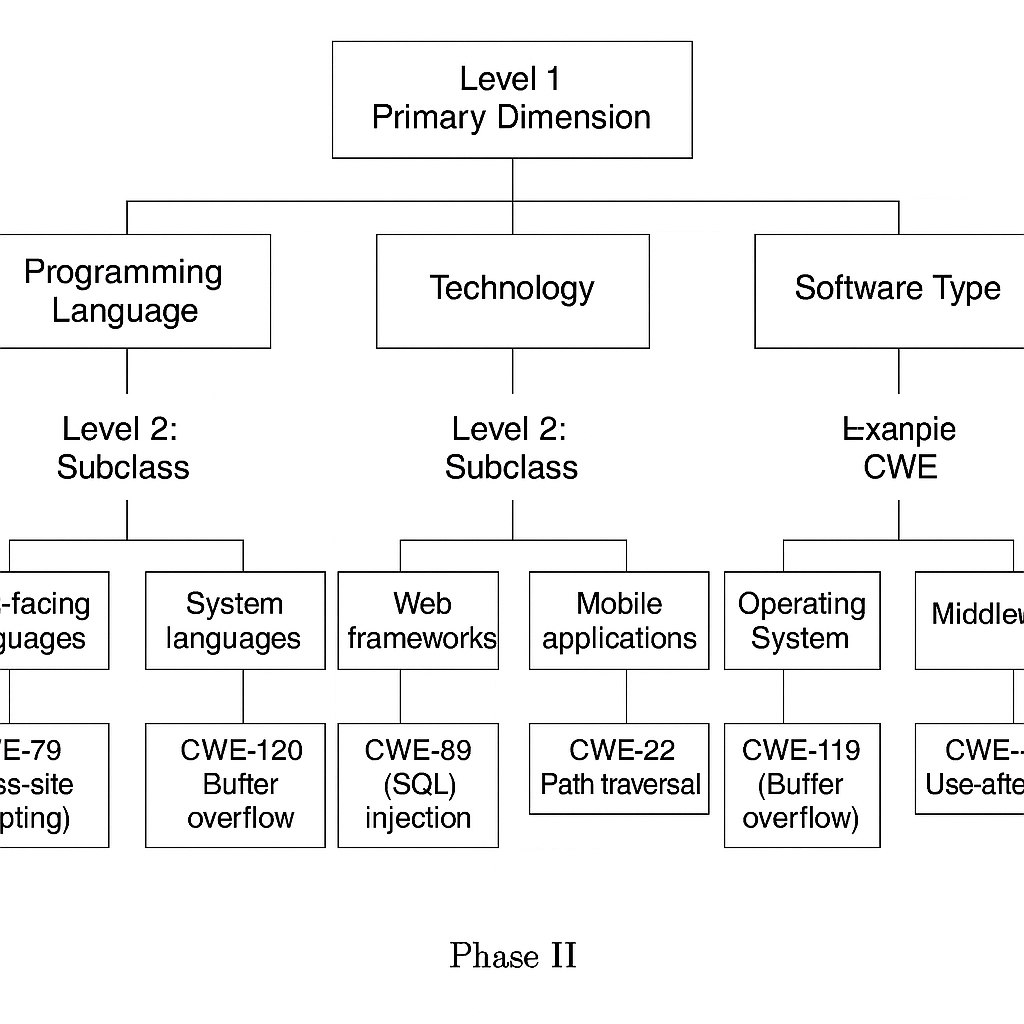
\includegraphics[width=0.55\textwidth]{figures/chapter_2/classification-hierarchy.png}
	\caption{Hierarchical classification}
	\label{fig:classification-hierarchy}
\end{figure}


Figure~\ref{fig:classification-hierarchy} (above) sketches the hierarchical classification derived in Phase III. Each Dimension branches into subclasses with illustrative CWE examples at the leaves. This taxonomy is rooted in the empirical data patterns uncovered and in prior taxonomies cited earlier. Through these steps, Phase III links the aggregated data back to our taxonomy framework, revealing how software vulnerabilities distribute across the multi-dimensional space. The resulting classification scheme provides a structured way to profile security faults, based both on existing knowledge (the taxonomies) and new insights from the data analysis.
